\documentclass[11pt]{article}
\usepackage[review]{acl}
\usepackage{times}
\usepackage{latexsym}
\usepackage{amsmath}
\usepackage{booktabs}
\usepackage{graphicx}
\usepackage{microtype}
\usepackage{url}
\usepackage{natbib}
\usepackage[hidelinks]{hyperref}

\title{GPS-Agent: A State-Graph Framework for Reducing Direct Answer-Giving in LLM-Based Mathematics Tutoring}

\author{Anonymous Submission}

\begin{document}
\maketitle
\begin{abstract}
Large language models can solve mathematics problems fluently, but this ability creates a pedagogical failure mode: the tutor gives the answer before the learner has reasoned through the problem. We present GPS-Agent, a stateful multi-agent tutoring framework that enforces a Guide--Practice--Solve protocol through graph-based routing. GPS-Agent is evaluated on a Vietnamese mathematics tutoring corpus with 5 student profiles, 45 probability/combinatorics questions, 225 human pilot sessions, and 810 annotated Guide/Practice/Solve turns, plus a controlled simulation suite comparing 100 GPS-Agent sessions against 100 single-agent baseline sessions over 25 questions. The primary result is pedagogical control rather than test-score improvement: GPS-Agent reduces direct-answer leakage from 54.0\% to 9.0\% (Fisher exact $p=3.83e-12$, odds ratio=0.084) and increases valid Guide--Practice--Solve trajectories from 0.0\% to 75.0\%. Secondary autonomy metrics do not yet show a reliable improvement, and failure analysis reveals a major remaining limitation: scaffolding pressure, where the tutor over-extends Practice turns. These results support the narrower claim that architectural constraints can reduce premature answer-giving, while longer-term learning gains require validated human pre/post studies.
\end{abstract}

\section{Introduction}
LLM-based tutors are attractive because they provide immediate, fluent, and individualized help. In mathematics education, however, the same fluency can undermine learning: a model often supplies a complete worked solution when the student needs a hint, a decomposition, or a prompt for self-explanation. We call this the \emph{Answer-Giving Trap}. It is not primarily an accuracy problem; the answer may be correct. It is a process-quality problem because the tutor may bypass the student's own reasoning.

This paper studies whether an architectural constraint can reduce that failure mode. GPS-Agent implements a three-phase protocol: \textbf{Guide}, where the tutor asks conceptual questions; \textbf{Practice}, where the student performs a sub-step; and \textbf{Solve}, where the tutor confirms the result and requests reflection. The protocol is implemented with specialized agents and a Supervisor over a state graph, rather than with a single prompt alone.

Our empirical claim is deliberately conservative. We do not claim that the current data prove long-term learning gain. Instead, we show that GPS-Agent improves two process-level outcomes that can be audited from tutoring logs: direct-answer leakage and phase validity. This positioning is important because the project includes both foundation logs and large augmented corpora; mixing them without clear labels would overstate the evidence.

\paragraph{Contributions.} We make three contributions. First, we formulate the Answer-Giving Trap as a measurable tutoring-system failure mode. Second, we introduce GPS-Agent, a state-graph framework for enforcing Guide--Practice--Solve sequencing. Third, we provide a reproducible evaluation pipeline that separates foundation data, controlled simulation, cross-model stress testing, and exploratory augmented data.

\section{Related Work}
Classical intelligent tutoring systems show that step-level feedback and cognitive scaffolding can outperform unguided worked solutions \citep{vanlehn2011relative,koedinger2006cognitive}. However, these systems often require domain-specific knowledge engineering. LLM-based tutors offer open-ended natural language interaction, but prior work has shown that pedagogical behavior is not guaranteed by fluency alone \citep{tack2022teacher,macina2023mathdial}.

The GPS protocol is motivated by faded scaffolding \citep{wood1976role} and the Zone of Proximal Development \citep{vygotsky1978mind}. It also relates to autonomy-supportive learning theories \citep{ryan2000self}: the tutor should create conditions for student reasoning rather than replace it. Multi-agent and graph-based LLM systems make it possible to encode such behavioral constraints as explicit routing policies rather than as soft instructions \citep{wu2023autogen}.

\section{GPS-Agent}
\subsection{Protocol}
GPS-Agent uses three pedagogical phases. In Guide, the tutor elicits prior knowledge and problem understanding without revealing the numerical solution. In Practice, the tutor asks for exactly one local computation or reasoning step. In Solve, the tutor verifies the final answer and asks for self-explanation. A session is phase-valid only if Solve occurs after at least one Guide and one Practice state.

\subsection{State-Graph Architecture}
The system stores message history, current phase, phase trace, student profile, and routing metadata in a shared state. A Supervisor classifies the next pedagogical action and dispatches to one of the specialized nodes. Compared with a single-agent prompt, this design makes the phase boundary explicit and auditable.

\subsection{Anti-Stagnation}
The current implementation includes a rule-based anti-stagnation signal. When the same phase repeats too many times without progress, the pipeline flags scaffolding pressure. In the present data, this signal is still a limitation rather than a solved component: GPS-Agent has a stall rate of 41.0\%, compared with 0.0\% for the baseline, because the baseline does not attempt multi-turn scaffolding.

\section{Data}
\subsection{Human Pilot}
The human pilot layer contains 5 student profiles and 45 probability/combinatorics questions, yielding 225 student-question sessions and 810 annotated turns. Phase counts are Guide=315, Practice=270, and Solve=225. This layer is used to define the problem setting and calibrate the GPS protocol.

\subsection{Controlled Evaluation Layer}
The primary comparison uses 100 GPS-Agent sessions and 100 single-agent baseline sessions over 25 unique questions and 4 student levels. This is the main layer used for statistical comparison because both conditions share the same schema.

\subsection{Cross-Model Stress Test}
We additionally evaluate 49 sessions using an independent Phi-3-style student simulator. This is not presented as a success-only result: it exposes higher leakage (42.9\%), high stall (79.6\%), and non-Vietnamese leakage (28.6\%).

\subsection{Data Quality Audit}
The extracted question bank contains 45 questions. The audit finds 15 missing answers and 43 questions with blank or malformed options. Therefore, correctness-based claims are restricted to validated subsets; the full 45-question pool is used primarily for tutoring-process analysis.

\section{Metrics}
\paragraph{Direct-answer leakage.} A session is flagged when the tutor gives answer-like or computation-heavy content before a valid Solve path is reached. This is the primary Answer-Giving Trap metric.

\paragraph{Phase validity.} A GPS trajectory is valid when Solve occurs only after Guide and Practice. Single-agent sessions have no explicit phase protocol and are therefore phase-invalid by design for this metric.

\paragraph{VAI and math density.} The Verifiable Autonomy Index (VAI) is the share of explicit mathematical expressions contributed by the student:
\begin{equation}
\mathrm{VAI} = \frac{M_{student}}{M_{student} + M_{tutor}}.
\end{equation}
Math density is the mean number of explicit mathematical expressions per student turn. These are secondary engagement indicators, not validated learning-gain metrics.

\section{Results}
\begin{table*}[t]
\centering
\small
\begin{tabular}{lrrrrr}
\toprule
System & $N$ & Leakage (\%) & Phase-valid (\%) & VAI & Stall (\%) \\
\midrule
GPS-Agent & 100 & 9.0 & 75.0 & 0.326 & 41.0 \\
Single-Agent & 100 & 54.0 & 0.0 & 0.320 & 0.0 \\
Cross-Model Phi-3 & 49 & 42.9 & 100.0 & 0.361 & 79.6 \\
\bottomrule
\end{tabular}
\caption{Main controlled evaluation. Leakage and phase validity are the primary process metrics. VAI is secondary and is not a significant GPS-Agent improvement in the current logs.}
\label{tab:main}
\end{table*}

Table~\ref{tab:main} shows the main controlled comparison. GPS-Agent reduces direct-answer leakage from 54.0\% to 9.0\%, a relative reduction of 83.3\% (Fisher exact $p=3.83e-12$). It also increases phase validity from 0.0\% to 75.0\% ($p=2.87e-33$). This supports the claim that a state-graph tutor can enforce pedagogical sequencing more reliably than a single-agent baseline.

\begin{figure}[t]
\centering
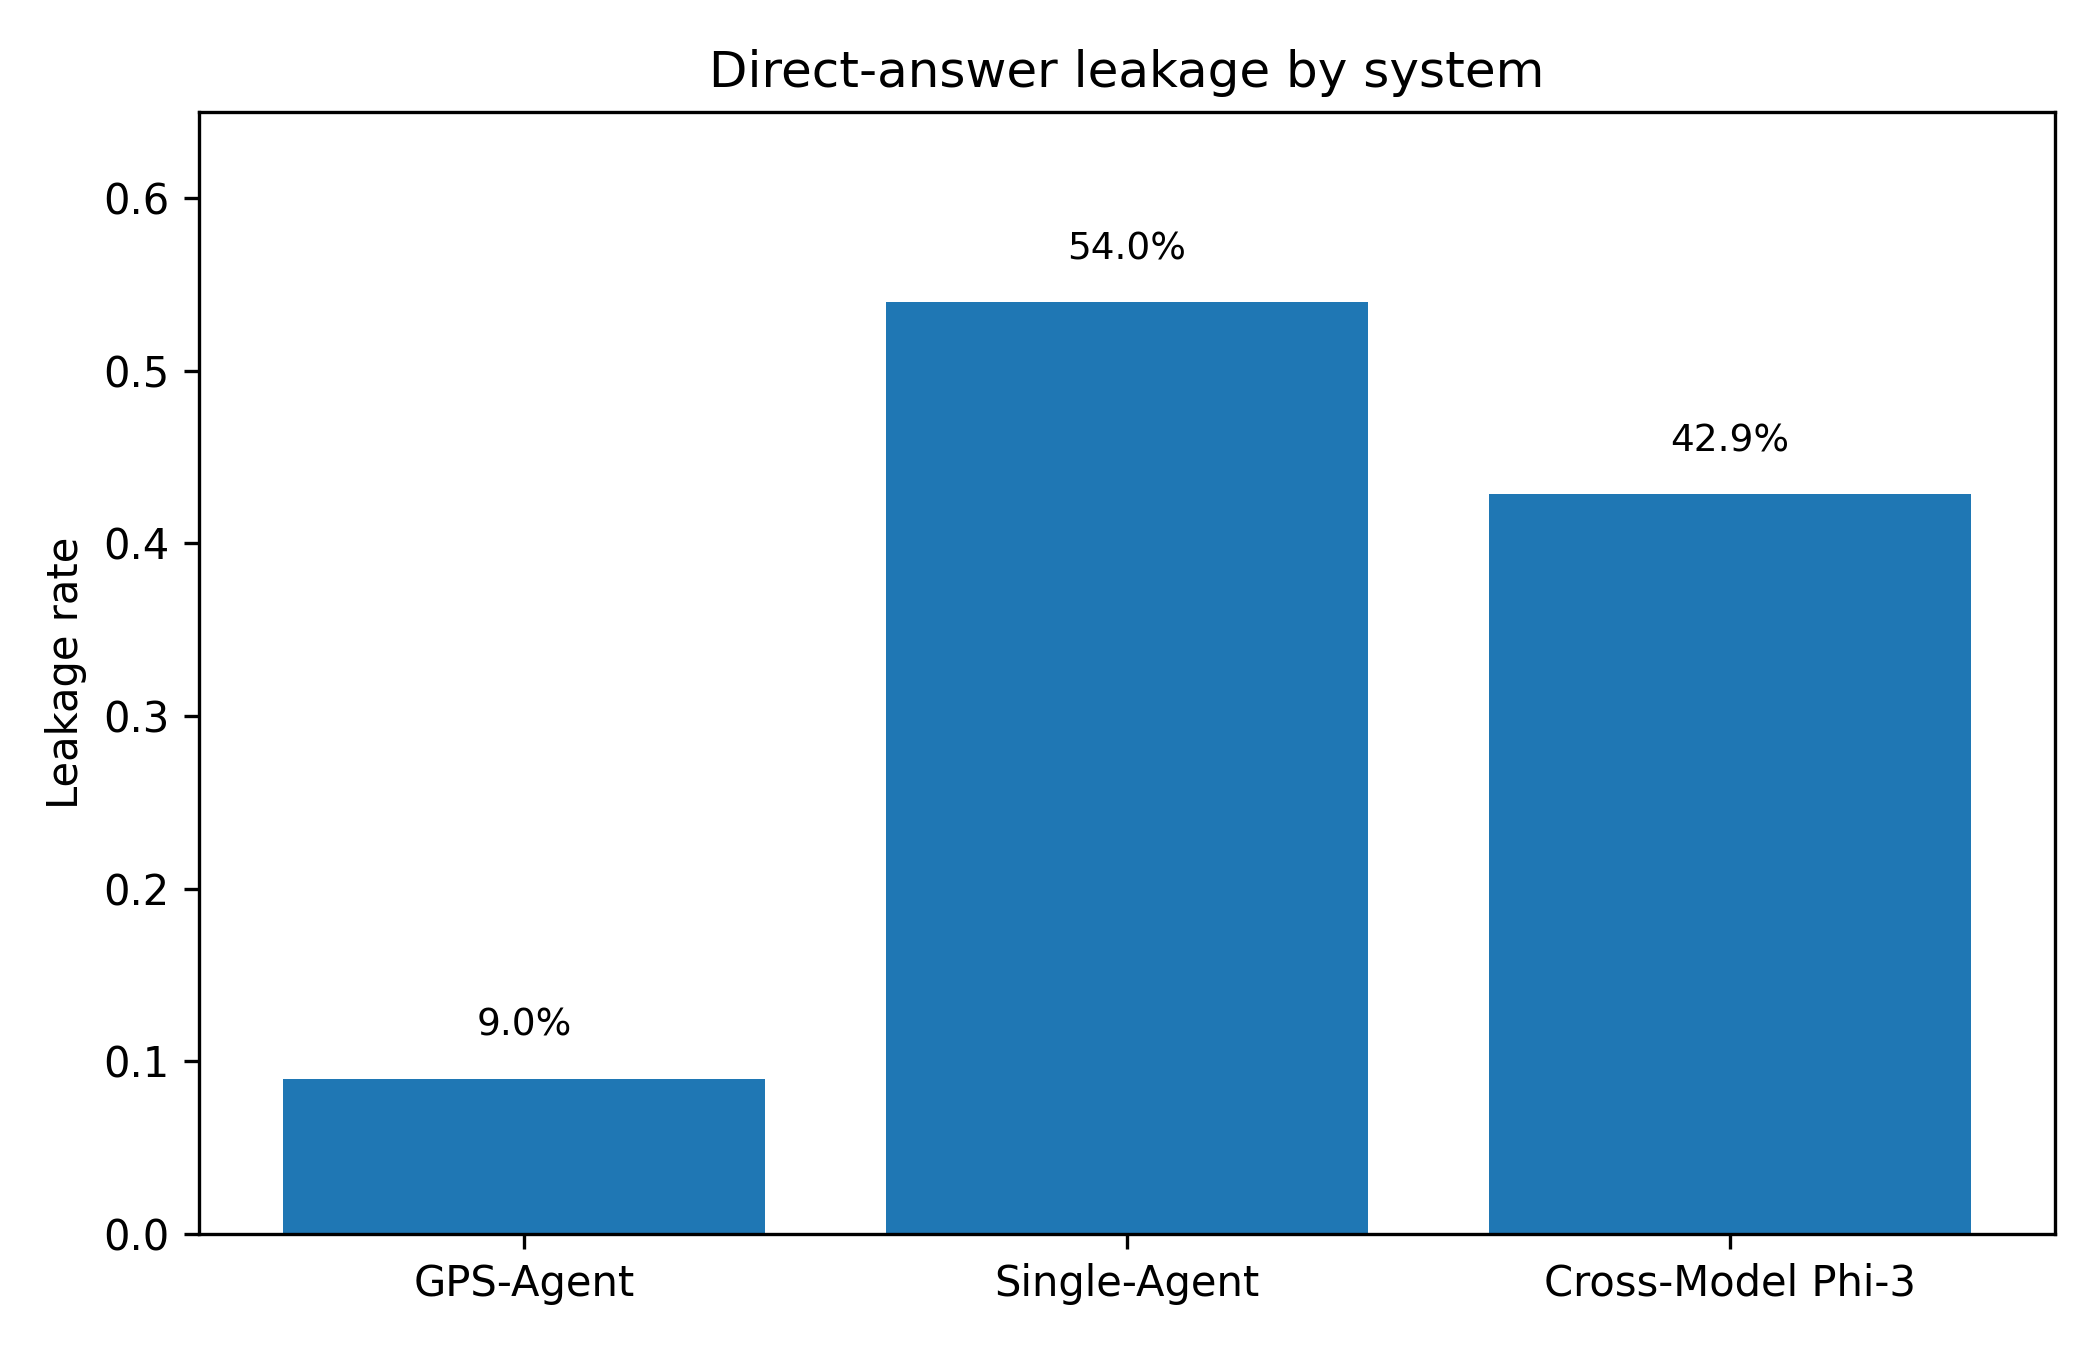
\includegraphics[width=\linewidth]{figures/fig_direct_answer_leakage.png}
\caption{Direct-answer leakage is substantially lower in GPS-Agent than in the single-agent baseline.}
\label{fig:leakage}
\end{figure}

The secondary autonomy metrics are more cautious. GPS-Agent obtains VAI=0.326, while the baseline obtains VAI=0.320; the difference is not statistically reliable ($p=0.870$, Cohen's $d=0.023$). Math density follows the same pattern and should not be used as a central claim without stronger human validation.

\begin{table}[t]
\centering
\small
\begin{tabular}{lrrrrr}
\toprule
Level & $N$ & Leak. & Valid & VAI & Stall \\
\midrule
Excellent & 25 & 20.0 & 84.0 & 0.311 & 52.0 \\
Good & 25 & 0.0 & 72.0 & 0.358 & 36.0 \\
Average & 25 & 8.0 & 80.0 & 0.293 & 40.0 \\
Weak & 25 & 8.0 & 64.0 & 0.341 & 36.0 \\
\bottomrule
\end{tabular}
\caption{GPS-Agent results by student level. Level labels are translated to English for submission readability.}
\label{tab:level}
\end{table}

\section{Failure Analysis}
The main failure mode is scaffolding pressure. GPS-Agent flags stall in 41.0\% of controlled sessions. This is expected for a tutor that tries to preserve student reasoning, but it is still pedagogically risky: excessive Practice turns may frustrate weaker or disengaged students. The cross-model stress test amplifies this issue, with stall=79.6\% and non-Vietnamese leakage=28.6\%.

The current IRR file should also be treated as a diagnostic rather than a validation result. Recomputed agreement is quadratic weighted kappa=nan over 100 paired ratings. We therefore do not claim substantial inter-rater agreement.

\section{Discussion}
The results support a focused architectural conclusion: GPS-Agent reduces premature answer-giving and makes pedagogical phase control auditable. This is weaker than claiming improved learning, but it is also more defensible. In educational NLP, process control is a necessary intermediate outcome: a tutor that cannot avoid giving away answers is unlikely to support independent problem solving.

The stall results reveal the next engineering target. A better Supervisor should distinguish productive struggle from unproductive stagnation. The next version should combine explicit student-state modeling, a frustration detector, and adaptive fading policies rather than relying only on consecutive-phase heuristics.

\section{Conclusion}
We presented GPS-Agent, a state-graph framework for pedagogically constrained LLM tutoring in mathematics. In controlled evaluation, GPS-Agent substantially reduces direct-answer leakage and improves Guide--Practice--Solve phase validity. However, VAI and math density do not yet provide strong evidence of learning improvement, and scaffolding pressure remains a major limitation. The current contribution is therefore best understood as a reproducible system paper on pedagogical process control, not as a completed learning-outcomes study.

\section{Limitations}
The foundation layer is small and should not be interpreted as a large-scale classroom trial. The controlled comparison uses LLM-as-student simulation, which cannot fully capture human affect, motivation, or long-term retention. The question bank requires further cleaning before correctness-based evaluation over all 45 questions. The IRR study must be rerun with calibrated human or carefully validated judge labels. Finally, the local LaTeX package included in this artifact is a compile-compatible fallback; authors should replace it with the official ACL style files for final submission.

\section{Ethics Statement}
GPS-Agent is designed to assist teachers rather than replace them. Any classroom deployment should obtain informed consent, protect student logs, and avoid using autonomy metrics as punitive student evaluations. Direct-answer leakage and stall alerts should be interpreted as system diagnostics and teacher-support signals.

\begin{thebibliography}{}
\bibitem[Koedinger and Corbett(2006)]{koedinger2006cognitive}
Koedinger, Kenneth R. and Corbett, Albert T. 2006.
\newblock Cognitive tutors: Technology bringing learning science to the classroom.
\newblock In \emph{The Cambridge Handbook of the Learning Sciences}.

\bibitem[Macina et~al.(2023)]{macina2023mathdial}
Macina, Jakub, Nico Daheim, Saurabh Srivastava, Philipp Mondorf, Katja Markert, Mrinmaya Sachan, and Mirella Lapata. 2023.
\newblock MathDial: A dialogue tutoring dataset with rich pedagogical properties grounded in math reasoning problems.
\newblock In \emph{Findings of EMNLP}.

\bibitem[Ryan and Deci(2000)]{ryan2000self}
Ryan, Richard M. and Edward L. Deci. 2000.
\newblock Self-determination theory and the facilitation of intrinsic motivation, social development, and well-being.
\newblock \emph{American Psychologist}, 55(1):68--78.

\bibitem[Tack and Piech(2022)]{tack2022teacher}
Tack, Anais and Chris Piech. 2022.
\newblock The AI Teacher Test: Measuring the pedagogical ability of Blender and GPT-3 in educational dialogues.
\newblock In \emph{Proceedings of EDM}.

\bibitem[VanLehn(2011)]{vanlehn2011relative}
VanLehn, Kurt. 2011.
\newblock The relative effectiveness of human tutoring, intelligent tutoring systems, and other tutoring systems.
\newblock \emph{Educational Psychologist}, 46(4):197--221.

\bibitem[Vygotsky(1978)]{vygotsky1978mind}
Vygotsky, Lev S. 1978.
\newblock \emph{Mind in Society: The Development of Higher Psychological Processes}.
\newblock Harvard University Press.

\bibitem[Wood et~al.(1976)]{wood1976role}
Wood, David, Jerome S. Bruner, and Gail Ross. 1976.
\newblock The role of tutoring in problem solving.
\newblock \emph{Journal of Child Psychology and Psychiatry}, 17(2):89--100.

\bibitem[Wu et~al.(2023)]{wu2023autogen}
Wu, Qingyun, Gagan Bansal, Jieyu Zhang, Yiran Wu, Beibin Li, Erkang Zhu, and others. 2023.
\newblock AutoGen: Enabling next-gen LLM applications via multi-agent conversation.
\newblock \emph{arXiv preprint arXiv:2308.08155}.
\end{thebibliography}
\end{document}
